\documentclass[12pt]{report}
\usepackage[italian]{babel}
\usepackage[most]{tcolorbox}
\usepackage{amsmath}
\usepackage{amsthm}
\usepackage{mathtools}
\usepackage{tabularx}
\usepackage{amssymb}
\usepackage{enumitem}
\usepackage{amsfonts}
\usepackage{centernot}
\usepackage{relsize}
\usepackage{mathrsfs}
\usepackage{bm}
\usepackage{xfrac}
\usepackage{lipsum}
\usepackage{bbm}
\usepackage{tikz}
\usepackage{cancel}
\usepackage{enumitem}
\usepackage{mathtools}
\usepackage{multicol}
\usepackage{float}
\usepackage{hyperref}
\usepackage{makecell}
\usepackage{listings}
\usepackage{xcolor}
\usepackage{pgfplots}
\usepackage{calligra}
\usepackage[toc,page]{appendix}
\usepackage{tikz}
\usepackage{yhmath}
\usetikzlibrary{angles, quotes, patterns}
\usepackage{circledsteps}
\date{}
\author{Alessandro Carella}
\title{Basi di dati}
\setcounter{chapter}{0}
\setlist[enumerate]{label*=\arabic*.}
\setlength{\parindent}{0pt}
\definecolor{brickred}{RGB}{182, 50, 28}
\definecolor{darkred}{RGB}{139, 0, 0}
\hypersetup{
	colorlinks=true,
	linkcolor=darkred,
	filecolor=darkred,
	urlcolor=darkred
}

\newcounter{theorem}
\newcounter{lemma}
\newcounter{corollary}
\newcounter{definition}
\newcounter{exercise}

\labelformat{theorem}{teorema #1}
\labelformat{lemma}{lemma #1}
\labelformat{corollary}{corollario #1}
\labelformat{definition}{definizione #1}
\labelformat{note}{nota #1}
\labelformat{example}{esempio #1}
\labelformat{exercise}{esercizio #1}

\newtcbtheorem[number within=chapter,use counter=theorem]{theorem}%
{Teorema}{arc=1mm,outer arc=1mm,colframe=cyan!55!black,fonttitle=\scshape,lefttitle=1mm,separator sign dash,description font=\bfseries,description delimiters={\flqq}{\frqq}}{th}

\newtcbtheorem[number within=theorem,use counter=corollary]{corollary}%
{Corollario}{arc=1mm,outer arc=1mm,colframe=cyan!55!black,fonttitle=\scshape,lefttitle=1mm,separator sign dash,description font=\bfseries,description delimiters={\flqq}{\frqq}}{cor}

\newtcbtheorem[number within=chapter,use counter=lemma]{lemma}%
{Lemma}{arc=1mm,outer arc=1mm,colframe=cyan!55!black,fonttitle=\scshape,lefttitle=1mm,separator sign dash,description font=\bfseries,description delimiters={\flqq}{\frqq}}{lem}

\newtcbtheorem[number within=chapter,use counter=definition]{definition}%
{Definizione}{arc=1mm,outer arc=1mm,colframe=green!55!black,fonttitle=\scshape,separator sign dash,description font=\bfseries,description delimiters={\flqq}{\frqq}}{def}

\newtcbtheorem[no counter]
{note}{Nota}{blanker,breakable,left=5mm,before skip=10pt,after skip=10pt,borderline west={2.5mm}{0pt}{red!55},coltitle=black,fonttitle=\bfseries}{note}

\newtcbtheorem[no counter]
{example}{Esempio}{blanker,breakable,left=5mm,before skip=10pt,after skip=10pt,borderline west={2.5mm}{0pt}{yellow!55},coltitle=black,fonttitle=\bfseries}{exa}

\newtcbtheorem[number within=section,use counter=exercise]
{exercise}{Esercizio}{blanker,breakable,left=5mm,before skip=10pt,after skip=10pt,borderline west={2.5mm}{0pt}{yellow!55},coltitle=black,fonttitle=\bfseries}{exe}

\newtcbtheorem[no counter]
{assignment}{Traccia}{blanker,breakable,left=5mm,before skip=10pt,after skip=10pt,borderline west={2.5mm}{0pt}{brickred!65},coltitle=black,fonttitle=\bfseries}{asg}
\tcolorboxenvironment{proof}{blanker,breakable,left=5mm,before skip=10pt,after skip=10pt,borderline west={2.5mm}{0pt}{cyan!55!black}}
\newcommand{\namerefl}[1]{%
	\bgroup
	\let\nmu\MakeLowercase
	\nameref{#1}\egroup}

\newcommand{\nmu}{}

\begin{document}
	{
		\let\cleardoublepage\clearpage
		\maketitle
		\tableofcontents
	}
	\chapter{Introduzione}
	\section{Sistema organizzativo, informativo e informatico}
	\begin{definition}{\nmu Sistema organizzativo}{sistema_organizzativo}
		Insieme di \textbf{risorse} e \textbf{regole} per lo svolgimento \textbf{coordinato} delle \textbf{attivita'} al fine di perseguire degli \textbf{scopi}
	\end{definition}
	\begin{definition}{\nmu Sistema informativo}{sistema_informativo}
		Un sistema informativo e':
		\begin{itemize}
			\item \textbf{Componente} di una \textbf{organizzazione} che gestisce \textbf{informazioni} (di interesse)
			\begin{itemize}
				\item e' parte del sistema organizzativo
				\item esegue/gestisce processi informativi ovvero processi che coinvolgono informazioni
				\item ogni organizzazione ha un sistema informativo, eventualmente non esplicitato nella struttura
				\item e' spesso di supporto ad altri sottosistemi ed e' da studiare nel contesto in cui e' inserito
				\item e' spesso suddiviso in sottosistemi piu' o meno fortemente integrati
			\end{itemize}
		\end{itemize}
		\end{definition}
		Esiste una dipendenza tra un sistema informativo e un \textbf{sistema informatico} per via dell'automatizzazione ed esistono organizzazioni la cui ragion d'essere e' la gestione di inforazioni e che operano da secoli. \\
		Un sistema informatico e' la porzione automatizzata del sistema informativo. \\
		Nel tempo c'e' stata un'evoluzione di sistemi informativi verso \textbf{razionalizzazione} e \textbf{standardizzazione} e delle procedure e dell'organizzazione delle informazioni. \\
		Una risorsa e' una qualsiasi fonte o mezzo che valga a fornire aiuto. \\
		\section{Gestione delle informazioni}
		Ci sono diverse modalita' di gestione delle informazioni:
		\begin{itemize}
			\item idee informali;
			\item linguaggio naturale;
			\item disegni, grafici, schemi;
			\item numeri e codici.
		\end{itemize}
		Inoltre, diversi sono i supporti sui quali memorizzare le informazioni:
		\begin{itemize}
			\item memoria umana;
			\item carta;
			\item dispositivi elettronici.
		\end{itemize}
		Nelle attivita' standardizzate di sistemi informativi complessi si e' giunti ad una organizzazione e codifica, ad esempio nei servizi anagrafici dalle registrazioni discorsive si e' giunti a:
		\begin{itemize}
			\item nome e cognome;
			\item estremi anagrafici;
			\item codice fiscale.
		\end{itemize}
		\section{Dati e informazioni}
			Nei sistemi informatici, per ragioni tecnlogiche e per la semplicita' dei meccanismi di gestione, il concetto di rappresentazione e codifica delle informazioni viene portato all'estremo: le informazioni vengono rappresentate per mezzo di dati che hanno bisogno di essere interpretati per fornire informazioni. E' difficile fare una distinzione tra dato e informazione ma per rappresentare in modo approssimativo il concetto possiamo dire che i dati da soli non hanno un significato ben definito ma una volta interpretati correttamente essi forniscono delle informazioni. Quindi l'informazione deriva da un processo di interpretazione e corellazione di dati, tutto cio' che produce variazione nel patrimonio conoscitivo di un soggetto e' informazione. \\
			Per fare un esempio di distinzione tra dato e informazione consideriamo la stringa 'BRINDISI  20 26 18', questi sono 4 dati e se correllati alla domanda 'Quali sono le temperature attuali, minime e massime di oggi?' allora i dati possono essere interpretati per fornire informazione e arricchire la conoscenza. \\
			I sistemi informatici si sono limitati a gestire solo i dati e le informazioni da esse estratte. \\
		\chapter{Sistemi di gestione di basi di dati}
			L'attenzione ai dati ha caratterizzato le applicazioni dell'informatica fin dalle sue origini, ma software dedicati alla loro gestione sono stati realizzati a partire dalla fine degli anni Sessanta. \\
			L'approccio convenzionale alla gestione dei dati sfrutta la presenza di archivi o \textit{file} per memorizzare i dati in modo persistente sulla memoria di massa. Un file consente di memorizzare e ricercare dati, ma fornisce semplici meccanismi di accesso e condivisione. Secondo questo approccio, le procedure scritte in un linguaggio di programmazione sono autonome, ciascuna utilizza uno o piu' file privati e dati di interesse sono replicati con ridondanza e possibilita' di incoerenza. \\
			Le basi di dati sono state concepite per superare questi inconvenienti, gestendo in modo integrato e flessibile le informazioni di interesse per diversi soggetti, limitando ridondanza e incoerenza.  \\
			Una base di dati e' una collezione di dati, di interesse per una o piu' applicazioni. \\
			Un \textit{sistema di gestione di basi di dati (Data Base Management System, DBMS)} e' un sistema software in grado di gestire collezione di dati che siano \textit{grandi}, \textit{condivise} e \textit{persistenti}, assicurando la loro \textit{affidabilita'} e \textit{privatezza}. Come ogni prodotto informatico, un DBMS deve essere \textit{efficiente} ed \textit{efficace}. Una base di dati e' una collezione di dati gestita da un DBMS. \\
			Chiariamo con precisione alcune caratteristiche dei DBMS e delle basi di dati:
			\begin{itemize}
				\item le basi di dati sono \textit{grandi}, nel senso che possono avere dimensioni molto maggiori della memoria centrale disponibile, di conseguenza i DBMS devono prevedere una gestione dei dati in memoria secondaria, con architettura molto sofisticate;
				\item le basi di dati sono \textit{condivise}, nel senso che diversi utenti e applicazioni possono accedervi secondo opportune modalita'. In questo modo si riduce la ridondanza dei dati e la conseguente inconsistenza in quanto se esistono copie diverse di uno stesso dato e' possibile che queste non siano uguali. Per garantire l'accesso condiviso ai dati, il DBMS dispone di un meccanismo apposito, detto \textit{controllo di concorrenza};
				\item le basi di dati sono \textit{persistenti}, cioe' hanno un tempo di vita non limitato a quello delle singole esecuzioni dei programmi che le utilizzano;
				\item i DBMS garantiscono \textit{affidabilita'}, cioe' la capacita' di conservare intatto il contenuto della base di dati in caso di malfunzionamenti hardware o software. A questo scopo i DBMS offrono funzionalita' di \textit{salvataggio} e \textit{ripristino};
				\item i DBMS garantiscono la \textit{privatezza} dei dati; ciasun utente, opportunamente riconosciuto, viene abilitato a svolgere solo determinate azioni sui dati, attraverso meccanismi di \textit{autorizzazione};
				\item i DBMS sono \textit{efficienti}, cioe' sono capaci di svolgere le operazioni utilizzando un insieme di risorse, tempo e spazio, che sia accettabile per gli utenti;
				\item i DBMS sono \textit{efficaci} in quanto sono capaci di rendere produttive le attivita' dei loro utenti.
			\end{itemize} 
			La gestione di collezioni di dati grandi e persistenti e' possibile anche con strumenti meno sofisticati dei DBMS, anche con i file, introdotti per gestire insiemi di dati localmente ad una specifica applicazione. I DBMS sono stati concepiti per estendere le funzioni del file system fornendo la possibilita' di accesso condiviso agli stessi dati da parte di piu' utenti e applicazioni. \\
			Inoltre, nei programmi tradizionali che accedono a file, ogni programma contiene una descrizione della struttura del file con rischi di incoerenza fra le varie descrizioni e i file stessi, nei DBMS, invece, c'e' una porzione di basi di dati, chiamata \textit{dizionario} o \textit{catalogo} che contiene una descrizione centralizzata dei dati che e' accessibile dai vari programmi. \\
			Diverse sono le tipologie di basi di dati e DBMS, come:
			\begin{itemize}
				\item basi di dati multimediali;
				\item data warehouse;
				\item GIS;
				\item basi di dati in tempo reale;
				\item basi di dati attive;
				\item NoSQL;
				\item Access;
				\item Oracle;
				\item PostgreSQL;
				\item MySql
			\end{itemize}
			e tante altre. \\
			\section{Modelli di dati}
			Un \textit{modello di dati} e' un insieme di concetti utilizzati per organizzare i dati di interesse e descriverne la struttura in modo che risulti comprensibile a un elaboratore. \\
			Ogni modello di dati fornisce \textit{meccanismi di strutturazione} analoghi ai costruttori di tipo dei linguaggi di programmazione, che permettono di definire nuovi tipi sulla base di tipi predefiniti e costruttori di tipo. \\
			Il \textit{modello relazionale} dei dati, il piu' diffuso, permette di definire tipi per mezzo del costruttore \textit{relazione}, che consente di organizzare i dati in insiemi di record a struttura fissa. Una relazione viene spesso rappresentata per mezzo di una tabella, le cui righe rappresentano dei record e le colonne corrispondono ai campi dei record, ad esempio: \\
			
			\begin{center}
			\begin{tabular}{|c|c|}
				\hline
				\multicolumn{2}{|c|}{Docenza} \\
				\hline
				Corso & NomeDocente \\
				\hline
				Basi di dati & Rossi \\
				Reti & Neri \\
				Linguaggi & Verdi \\
				\hline
			\end{tabular}
			\end{center}
			Oltre al modello relazionale sono stati definiti altri tipi di modelli:
			\begin{itemize}
				\item il \textit{modello gerarchico} basato sull'uso di strutture ad albero;
				\item il \textit{modello reticolare} basato sull'uso di grafi;
				\item il \textit{modello a oggetti}, sviluppato come evoluzione del modello relazionale che estende alle basi di dati il paradigma di programmazione ad oggetti;
				\item il \textit{modello XML} sviluppato come rivisitazione del modello gerarchico, in cui i dati vengono presentati assieme alla loro descrizione e non devono sottostare rigidamente a un'unica struttura logica;
				\item modelli semi-strutturati e flessibili, sviluppati nel contesto dei sistemi NoSQL che cercano di superare alcune limitazioni dei sistemi relazionali in termini di prestazioni e di rigidita' di organizzazione.
			\end{itemize}
			I modelli dei dati vengono detti \textit{logici} per sottolineare il fatto che le strutture utilizzate pur essndo astratte riflettono una particolare organizzazione (ad albero, grafo, ecc.). Piu' recentemente ai modelli logici, sono stati introdotti i modelli \textit{concettuali} utilizzati per descrivere i dati indipendenmente dalla scelta del modello logico. Il loro nome deriva dal fatto che essi tendono a descrivere i \textit{concetti} del mondo reale e vengono usati nella fase preliminare del processo di progettazione di basi di dati.
			\subsection{Schemi e istanze}
			Nelle basi di dati esiste una parte invariante nel tempo, detto \textit{schema} della base di dati, costituita dalle caratteristiche dei dati, e una parte variabile nel tempo, detta \textit{istanza} o \textit{stato} della base di dati, costituita dai valori effettivi. Lo schema di una relazione e' costituito dalla sua intestazione, ad esempio:
			\[
			Docenza(Corso, NomeDocente)
			\]
			Le righe della tabella, invece, variano nel tempo, l'istanza di una relazione e' costituita dall'insieme delle sue righe,
			\subsection{Livelli di astrazione nei DBMS}
			La notazione di modello descritta in precedenza puo' essere sviluppata tenendo presente di altri fattori nella descrizione dei dati. In particolare, esiste un'architettura standard per DBMS articolata su tre lvielli, detti: \textit{esterno}, \textit{logico} e \textit{interno} e per ogni livello esiste uno schema. 
			\begin{itemize}
				\item Lo \textit{schema logico} costituisce una descrizione dell'intera basi di dati per mezzo del modello logico adottato dal DBMS;
				\item Lo \textit{schema interno} costituisce la rappresentazione dello schema logico per mezzo di strutture fisiche di memorizzazione, ad esempio una relazione puo' essere realizzata tramite file sequenziale, file hash o altri approcci;
				\item Uno \textit{schema esterno} costituisce la descrizione di una porziona della base di dati di interesse, per mezzo del modello logico.
			\end{itemize}
			Nei sistemi moderni il livello esterno non e' esplicitamente presente, ma e' possibile definire relazioni derivate, o \textit{viste}.
			\subsection{Indipendenza dei dati}
			L'architettura a livelli cosi' definita garantisce l'\textit{indipendenza dei dati} che e' la principale prorieta' dei DBMS. L'indipendenza dei dati permette a utenti e programmi applicativi che utlizzano una base di dati di interagire a un elevato livello di astrazione, cioe' prescinde dai dettagli realizzativi. \\
			L'indipendenza dei dati puo' essere caratterizzata come indipendenza fisica e logica:
			\begin{itemize}
				\item l'\textit{indipendenza fisica} consente di interagire con il DBMS in modo indipendente dalla struttura fisica dei dati. E' possibile modificare le strutture fisiche, come le modalita' di orgaizzazione dei file gestiti dal DBMS, senza influire sulle descrizioni dei dati ad alto livello e quindi sui programmi che utilizzano i dati.
				\item l'\textit{indipendenza logica} consente di interagire con il livello esterno della base di dati in modo indipendente dal livello logico. Ad esempio, e' possibile aggiungere uno schema esterno in base alle esigenze di un nuovo utente o modificare uno schema esterno senza dover modificare lo schema logico e quindi l'organizzazione fisica dei dati.
			\end{itemize}
			Gli accessi alla base di dati avvengono solo attraverso il livello esterno ed e' il DBMS che traduce le operazioni in termini dei livelli sottostanti.
			\section{Linguaggi e utenti delle basi di dati}
			I DBMS sono caratterizzati dalla presenza di diversi linguaggi per la gestione dei dati e dalla presenza di molteplici utenti. 
			\subsection{Linguaggi per basi di dati}
			E' possibile effettuare diverse operazioni su un DBMS, in particolare quelle relative agli schemi e alle istanze. I linguaggi per basi di dati si distinguono in due categorie:
			\begin{itemize}
				\item \textit{linguaggi di definizione dei dati (Data Definition Language, DDL)}, utilizzati per definire gli schemi logici, esterni e fisici e le autorizzazioni per l'accesso;
				\item \textit{linguaggi di manipolazione dei dati (Data Manipulation Language, DML)}, utilizzati per l'interrogazione e l'aggiornamento delle istanze di basi di dati.
			\end{itemize}
			L'accesso ai dati puo' essere effettuato con varia modalita':
			\begin{itemize}
				\item tramite linguaggi testuali interattivi, come il linguaggio SQL. Ad esempio, possiamo definire la struttura della relazione \textit{Docenza}, sottoponendo a un interprete SQL la seguente istruzione che appartiene al DDL:
				\begin{lstlisting}
create table Docenza (
	Corso	    character(20),
	NomeDocente character(30)
)
				\end{lstlisting}
				\item tramite comandi simili a quelli interattivi immersi in linguaggi di programmazione. Questi linguaggi di programmazione si dicono \textit{linguaggi ospite} perche' ospitando comandi scritti nel linguaggio per basi di dati. Questo approccio si utilizza spesso nella realizzazione di applicazioni parametriche e di farle eseguire ad un utente che non conosce SQL;
				\item tramite comandi simili a quelli interattivi immersi in linguaggi di sviluppo ad hoc, spesso con funzionalita' specifiche;
				\item tramite interfacce amichevoli che permettono di sintetizzare interrogazioni senza usare un linuaggio testuale.
			\end{itemize}
			\subsection{Utenti e progettisti}
			Diverse categorie di persone possono interagire con una base di dati o con un DBMS.
			\begin{itemize}
				\item l'\textit{amministratore della base di dati (DataBase Administrator, DBA)} e' la persona o gruppo di persone responsabile della progettazione, controllo e amministrazione della base di dati, l'acquisizione di software e risorse hardware e controlla l'efficienza delle operazioni;
				\item i \textit{progettisti e programmatori di applicazioni} definiscono e realizzano i programmi che accedono alla base di dati. Essi utilizzano i linguaggi DML;
				\item gli \textit{utenti} utilizzano la base di dati per le proprie attivita' e gli utenti si dividono in due categorie:
				\begin{itemize}
					\item \textit{utenti finali} o \textit{terminalisti} che utilizzano \textit{transazioni}, cioe' programmi che realizzano attivita' predefinite e di frequenza elevata;
					\item \textit{utenti casuali} in grado di impiegare i linguaggi interattivi per l'accesso alla base di dati, formulando interrogazioni o aggiornamenti di vario tipo. Essi possono essere specializzati e interagire frequentemente con la base di dati.
				\end{itemize}
			\end{itemize}
			\section{Vantaggi e svantaggi dei DBMS}
			Dei DBMS possiamo elencare i seguenti vantaggi:
			\begin{itemize}
				\item I DBMS permettono di considerare i dati come una risorsa comune di un'organizzazione, a disposizione di tutte le sue componenti;
				\item la base di dati fornisce un modello unificato e preciso dalla parte del mondo reale di interesse per l'organizzazione;
				\item utilizzando un DBMS e' possibile un controllo centralizzato dei dati, che puo' essere arricchito da forme di standardizzazione e beneficiare di "economie di scala";
				\item la condivisione permette di ridurre ridondanze e inconsistenze;
				\item l'indipendenza dei dati, fornisce lo sviluppo di applicazioni piu' flessibili e facilmente modificabili.
			\end{itemize}
			In casi di applicazioni con uno o pochi utenti, senza accessi concorrenti possono essere utlilizzati file rispetto ai DBMS in quanto puo' risultare sconveniente.
		\chapter{Metodologie e modelli per il progetto}
		\section{Il ciclo di vita dei sistemi informativi}
		La progettazione di una basd di dati costituisce solo una delle componenti del processo di sviluppo di un sistema informativo complesso e va quindi inquadrata in un contesto piu' ampio, quello del \textit{ciclo del vita} dei sistemi informativi. \\
		Il ciclo di vita di un sistema informativo comprende le seguenti attivita'.
		\begin{figure}[H]
			\centering
			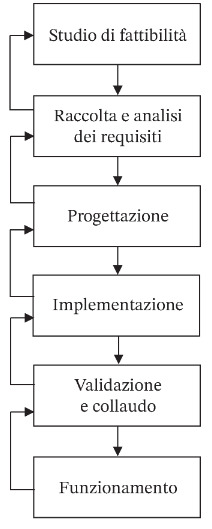
\includegraphics[width=0.2\textwidth]{ciclo_di_vita}
		\end{figure}
		\begin{itemize}
			\item \textbf{Studio di fattibilita'}. Serve a definire, nel modo piu' preciso possibile, i costi delle varie alternative possibili e a stabilire le priorita' di realizzazione delle varie componenti del sistema.
			\item \textbf{Raccolta e analisi dei requisiti}. Consiste nell'individuazione e nello studio delle proprieta' e delle funzionalita' che il sistema informativi dovra' avere. Questa fase richiede un'iterazione con gli utenti del sistema e produce una descrizione completa, ma informale, dei dati coinvolti e delle operazioni su di essi. Vengono inoltre stabiliti i requisiti software e hardware del sistema informativo.
			\item \textbf{Progettazione}. Si divide generalmente in \textit{progettazione di dati} e \textit{progettazione delle applicazioni}. Nella prima si individua la struttura e l'organizzazione che i dati dovranno avere, nell'altra si definiscono le caratteristiche dei programmi applicativi. \\
			Le due attivita' sono complementari e possono procedere in parallelo o in cascata. Le descrizioni dei dati e delle applicazioni prodotti sono formali e fanno riferimento a specifici modelli.
			\item \textbf{Implementazione}. Consiste nella realizzazione del sistema informativo secondo la struttura e le caratteristiche definite nella fase di progettazione. Viene costruita e popolata la base di dati e viene prodotto il codice dei programmi.
			\item \textbf{Validazione e collaudo}. Serve a verificare il corretto funzionamento e la qualita' del sistema informativo. La sperimentazione deve prevedere tutte le condizioni operative.
			\item \textbf{Funzionamento}. In questa fase il sistema informativo diventa operativo ed esegue i compiti per i quali era stato progettato. Se non si verificano malfunzionamenti delle funzionalita' del sistema, questa attivita' richiede solo operazioni di gestione e manutenzione.
		\end{itemize}
		Il processo non e' quasi mai strettamente sequenziale in quanto, durante l'attivita' di una delle attivita' citate, bisogna rivedere decisioni prese nell'attivita' precedente. Inoltre, oltre alle attivita' descritte, si aggiunge quella di \textit{prototipizzazione}, che consiste nell'uso di specifici strumenti software pe la realizzazione rapida di una versione semplificata del sistema informativo, con la quale sperimentare le sue funzionalita'. La verifica del prototipo puo' portare ad un'eventuale revisione del progetto. \\
		I dati hanno un ruolo centrale nei sistemi informativi e questo giustifica uno studio autonomo relativo alla progettazione delle basi di dati. 
		\section{Metodologie di progettazione e basi di dati}
		Bisogna precisare cosa si intende per \textit{metodologia di progettazione} e quali sono le propriota' che deve garantire. Una metodologia di progettazione consiste in:
		\begin{itemize}
			\item una \textit{decomposizione} dell'interva attivita' di progetto in passi successivi indipendenti tra loro;
			\item una serie di \textit{strategie} da seguire nei vari passi e alcuni \textit{criteri} per la scelta in caso di alternative;
			\item alcuni \textit{modelli di riferimento} per descrivere i dati di ingresso e uscita delle varie fasi. 
		\end{itemize}
		Le proprieta' che una metodologie deve garantire sono principalmente:
		\begin{itemize}
			\item la \textit{generalita'} rispetto alle applicazioni e ai sistemi di gioco (e quindi la possibilita' di utilizzo indipendentemente dal problema allo studio e dagli strumenti a disposizione);
			\item la \textit{qualita' del prodtto} in termini di correttezza, completezza ed efficienza rispetto alla risorse impiegato;
			\item la \textit{facilita' d'uso} delle strategie e dei modelli di riferimento. 
		\end{itemize}
		Nelle basi di dati, nel corso degli anni si e' consolidata una metodologia di progetto che e' articolata in tre fasi principali da effettuare in cascata. Questa metodologia separa le decisioni relative a \textit{cosa} rappresentare in una base di dati, da quelle relative a \textit{come} farlo.
		\begin{figure}[H]
			\centering
			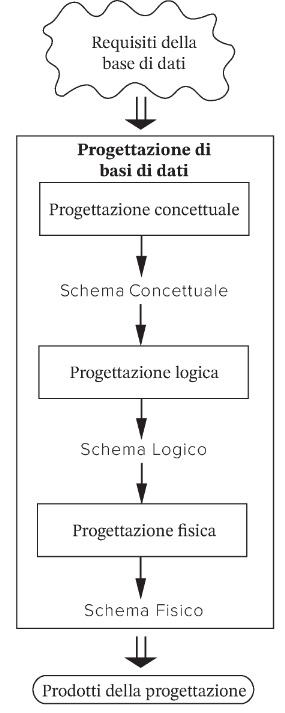
\includegraphics[width=0.5\textwidth]{progettazione_db}
		\end{figure}
		\begin{itemize}
			\item \textbf{Progettazione concettuale}. Il prodotto di questa fase viene chiamato \textit{schema concettuale} e fa riferimento a un \textit{modello concettuale} dei dati. I modelli concettuali ci consentono di descrivere l'organizzazione dei dati a un alto livello di astrazione senza tenere conto degli aspetti implementativi. In questa fase, il progettista deve cercare di rappresentare il \textit{contenuto informativo} delle base di dati non pensando a dettagli implementativi. Il modello concettuale piu' noto e' il modello \textbf{Entity-Relationship}.
			\item \textbf{Progettazione logica}. Consiste nella traduzione dello schema concettuale definito nella fase precedente, adottando il modello di rappresentazione di dati del DBMS a disposizione. Il prodotto di questa fase viene denominato \textit{schema logico} delle base di dati e fa riferimento a un \textit{modello logico} dei dati. Il modello logico ci consente di descrivere i dati prescindendo ancora da dettagli fisici, ma concreta perche' disponile nei sistemi di gestione di basi di dati. In questa fase, le scelte progettuali si basano su criteri di ottimizzazione delle operazioni da effettuare sui dati. Inoltre, si fa uso di tecniche formali di verifica della qualita' dello schema logico ottenuto. Nel caso del modello relazione dei dati, la tecnica usata e' quella della \textit{normalizzazione}
			\item \textbf{Progettazione fisica}. In questa fase lo schea logico viene completato con la specifica dei parametri fisici di memorizzazione dei dati. Il prodotto di questa fase viene chiamato \textit{schema fisico} e fa riferimento a un \textit{modello fisico} dei dati che dipende dal DBMS scelto e si basa sui criteri di organizzazione fisica dei dati.
		\end{itemize}
		Analizziamo come i requisiti della base di dati vengono utilizzati nelle varie fasi della progettazione. Dobbiamo prima distinguere le \textit{specifiche sui dati} che riguardano il contenuto della base di dati, e \textit{specifiche sulle operazioni} che riguardano l'uso che utenti e applicazioni fanno della base di dati. Nella progettazione concettuale si fa uso delle specifiche sui dati mentre le specifiche sulle operazioni servono solo a verificare che lo schema concettuale sia completo, cioe' che contenga le informazioni necessarie per eseguire tutte le operazioni previste. 
		\chapter{Il modello relazionale}
		\section{Struttura del modello relazionale}
		\subsection{Modelli logici nei sistemi di basi di dati}
		Il \textit{modello relazionale} si basa su due concetti fondamentali, quello di \textit{relazione} e \textit{tabella}. \\
		La nozione di \textit{relazione} proviene dalla teoria di insiemi in matematica mentre il concetto di \textit{tabella} e' intuitivo. \\
		Il modello relazionale risponde al requisito d'indipendenza dei dati che prevede una distinzione, nella descrizione dei dati, fra il livello \textit{fisico} e il livello \textit{logico}; gli utenti che accedono ai dati e i programmatori che sviluppano le applicazioni fanno riferimento solo al livello logico e i dati descritti al livello logico sono concretamente organizzati per mezzo di strutture fisiche, ma non e' necessario conoscerne i dettagli per accedervi. Invece, il modello reticolare e gerarchico, includevano riferimenti alla struttura realizzativa, attraverso l'uso di puntatori e l'ordinamento fisico dei dati. \\
		Il termine \textit{relazione} viene utilizzato in tre accezioni:
		\begin{enumerate}
			\item \textit{relazione matematica} secondo la definizione della teoria degli insiemi;
			\item \textit{relazione} secondo la definizione del modello relazionale che presenta differenze a quella della teoria degli insiemi;
			\item \textit{relazione} come traduzione di \textit{relationship} costrutto del modello concettuale \textit{Entita'-Relazione} utilizzato per descrivere legami tra entita' del mondo reale.
		\end{enumerate}
		\subsection{Relazioni e tabelle}
		In matematica, dati due insiemi $\mathcal{D}_1$ e $\mathcal{D}_2$, si chiama \textit{prodotto cartesiano} di $\mathcal{D}_1$ e $\mathcal{D}_2$, l'insieme di coppie ordinate $(v_1, v_2)$, tali che $v_1$ e' un elemento di $\mathcal{D}_1$ e $v_2$ e' un elemento di $\mathcal{D}_2$. 
		\begin{example}{\nmu Prodotto cartesiano}{prod_cartesiano}
			Dati due insiemi $A = \{1, 2, 3, 4\}$ e $B = \{a, b\}$, il prodotto cartesiano e':
			\[
			A \times B = \{(1, a), (1, b), (2, a), (2, b), (3, a), (3, b), (4, a), (4, b)\}
			\]
			ovvero l'insieme di tutti le possibili coppie dove il primo elemento appartiene ad $A$ e il secondo a $B$.
		\end{example}
		Una \textit{relazione matematica} sugli insiemi $\mathcal{D}_1$ e $\mathcal{D}_2$, detti \textit{domini} della relazione, e' un sottoinsieme di $\mathcal{D}_1 \times \mathcal{D}_2$. \\
		Le relazioni possonoe essere espresse graficamente sotto forma tabellare, ad esempio prendendo spunto dall'esempio del \namerefl{exa:prod_cartesiano}, possiamo rappresentare la relazione cosi: \\
		\begin{center}
			\begin{tabular}{|c|c|}
			\hline
			1 & a \\
			1 & b \\
			2 & a \\
			2 & b \\
			4 & a \\
			4 & b \\
			\hline
		\end{tabular}
		\hspace{2cm}
		\begin{tabular}{|c|c|}
			\hline
			1 & a \\
			1 & b \\
			4 & b \\
			\hline
		\end{tabular}
		\end{center}
	Le definizioni di prodotto cartesiano e relazione date precedentemente hanno fatto riferimento a due insiemi, ma possono essere generalizzate rispetto al numero di insiemi. Dati $n > 0$ insiemi $\mathcal{D}_1, \mathcal{D}_2, \dots, \mathcal{D}_n$, anche non distinti, il prodotto cartesiano di $\mathcal{D}_1 \times \mathcal{D}_2 \times \dots \times \mathcal{D}_n$ e' costituito dalle $n$-uple $(v_1, v_2, \dots, v_-n)$ tali che $v_1 \in \mathcal{D}_i \quad 1 \leq i \leq n$. \\
	Una relazione matematica sui domini $\mathcal{D}_1$, $\mathcal{D}_2$, $\dots$, $\mathcal{D}_n$ e' un sottoinsieme del prodotto cartesiano $\mathcal{D}_1 \times \mathcal{D}_2 \times \dots \times \mathcal{D}_n$. Il numero delle $n$ componenti del prodotto cartesiano viene detto \textit{grado} del prodotto cartesiano e della relazione. Il numero di elementi della relazione viene detto \textit{cardinalita'} della relazione.
	\subsection{Relazioni con attributi}
	Una relazione matematica e' un insieme di $n$-uple ordinate $(v_1, v_2, \dots, v_n)$ ove $v_1 \in \mathcal{D}_1$, $v_2 \in \mathcal{D}_2, \dots$, $v_n \in \mathcal{D}_n$. Ciascuna $n$-upla contiene dati fra loro collegati, stabilisce un legame fra loro, ad esempio una $n$-upla siffatta: "Juventus, Lazio, 3, 1" indica che il risultato della partita tra Juventus e Lazio e' 3 a 1. \\
	Una relazione e' un insieme quindi:
	\begin{itemize}
		\item non e' definito un ordinamento fra le $n$-uple;
		\item le $n$-uple di una relazione sono distinte l'una dall'altra, in quanto tra gli elementi di un insieme non ce ne possono essere due uguali fra loro.
	\end{itemize}
	Ciascuna $n$-upla e', al proprio interno, \textit{ordinata}: l'i-esimo valore di ciascuna proviene dall'i-esimo dominio. L'ordinamento appena descritto corrisponde ad una caratteristica insoddisfacente del concetto di relazione matematica rispetto alla possibilita' di organizzare e utilizzare i dati. Infatti, in vari contesti dell'informatica, si tende a privilegiare notazioni \textit{non-posizionali} rispetto a quelli posizionali: si tende a utilizzare quelli posizionali solo quando l'ordinamento corrisponde ad una esigenza intrinseca, come accade nei problemi di natura matematica, in cui gli array permettono di rappresentare in modo ovvio vettori e matrici. Le basi di dati, invece, hanno una struttura che si puo' ricondurre a quella dei record. Nel caso dei record, ad ogni campo, e' associato un nome e allo stesso modo, ad ogni dominio possiamo associare un nome detto \textit{attributo} che descrive il ruolo svolto dal dominio. Per esempio, nella relazione precedente delle squadre, possiamo usare nomi come "SquadraCasa, SquadraOspite, RetiCasa, RetiOspite". \\
	Modificando la definizione di relazione con l'introduzione degli attributi e quindi l'ordinamento degli attributi risulta irrilevante, non e' piu' necessario parlare di primo dominio, secondo dominio ecc. \\
	Per formalizzare i concetti, indichiamo con $\mathcal{D}$ l'insieme dei domini e specifichiamo la corrispondenza fra attributi e domini, nell'ambito di una relazione, per mezzo di una funzione $dom:\ X \to \mathcal{D}$, che associa a ciascun attributo $A \in X$ un dominio $dom(A) \in \mathcal{D}$. Poi diciamo che una \textit{tupla} su un insieme di attributi $X$ e' una funzione $t$ che associa a ciascun attributo $A \in X$ un valore del dominio $dom(A)$. Quindi una \textit{relazione} su $X$ e' un insieme di tuple su $X$. La differenza nella definzione precedente sta nel fatto che gli elementi delle tuple sono indivuati per mezzo degli attributi e non per posizione. \\
	Se $t$ e' una tupla su $X$ e $A$ un attributo nell'insieme $X$ allora $t[A]$ indica il valore di $t$ su $A$, ad esempio:
	\[
	t[SquadraOspite] = Lazio
	\]
	\subsection{Relazioni e basi di dati}
	Una base di dati e' costituita da piu' relazioni, le cui tuple, contengono valori comuni per stabilire delle corrispondenze. Ad esempio date le seguenti relazioni:
	\begin{center}
		
		\textbf{Studenti}
		
		\vspace{0.5cm}
		
		\begin{tabular}{|c|c|c|c|c|}
			\hline
			\textbf{Matricola} & \textbf{Cognome} & \textbf{Nome} & \textbf{Data di nascita} \\
			\hline
			276545 & Rossi & Maria & 25/11/2000 \\
			485745 & Neri & Anna & 23/04/2001 \\
			200768 & Verdi & Fabio & 12/02/2001 \\
			587614 & Rossi & Luca & 10/10/2000 \\
			937653 & Bruni & Mario & 01/12/2000 \\
			\hline
		\end{tabular}
		
		\vspace{1.5cm}
		
		\begin{minipage}[t]{0.45\textwidth}
			\centering
			\textbf{Esami}
			
			\vspace{0.5cm}
			
			\begin{tabular}{|c|c|c|}
				\hline
				\textbf{Studente} & \textbf{Voto} & \textbf{Corso} \\
				\hline
				276545 & 28 & 01 \\
				276545 & 27 & 04 \\
				937653 & 25 & 01 \\
				200768 & 24 & 04 \\
				\hline
			\end{tabular}
		\end{minipage}
		\hfill
		\begin{minipage}[t]{0.45\textwidth}
			\centering
			\textbf{Corsi}
			
			\vspace{0.5cm}
			
			\begin{tabular}{|c|c|c|}
				\hline
				\textbf{Codice} & \textbf{Titolo} & \textbf{Docente} \\
				\hline
				01 & Analisi & Giani \\
				03 & Chimica & Melli \\
				04 & Chimica & Belli \\
				\hline
			\end{tabular}
		\end{minipage}
		
	\end{center}
	\begin{center}
		
		\textbf{Studenti}
		
		\vspace{0.5cm}
		
		\begin{tabular}{|c|c|c|c|c|}
			\hline
			\textbf{Matricola} & \textbf{Cognome} & \textbf{Nome} & \textbf{Data di nascita} \\
			\hline
			276545 & Rossi & Maria & 25/11/2000 \\
			485745 & Neri & Anna & 23/04/2001 \\
			200768 & Verdi & Fabio & 12/02/2001 \\
			587614 & Rossi & Luca & 10/10/2000 \\
			937653 & Bruni & Mario & 01/12/2000 \\
			\hline
		\end{tabular}
		
		\vspace{1.5cm}
		
		\begin{minipage}[t]{0.45\textwidth}
			\centering
			\textbf{Esami}
			
			\vspace{0.5cm}
			
			\begin{tabular}{|c|c|c|}
				\hline
				\textbf{Studente} & \textbf{Voto} & \textbf{Corso} \\
				\hline
				276545 & 28 & 01 \\
				276545 & 27 & 04 \\
				937653 & 25 & 01 \\
				200768 & 24 & 04 \\
				\hline
			\end{tabular}
		\end{minipage}
		\hfill
		\begin{minipage}[t]{0.45\textwidth}
			\centering
			\textbf{Corsi}
			
			\vspace{0.5cm}
			
			\begin{tabular}{|c|c|c|}
				\hline
				\textbf{Codice} & \textbf{Titolo} & \textbf{Docente} \\
				\hline
				01 & Analisi & Giani \\
				03 & Chimica & Melli \\
				04 & Chimica & Belli \\
				\hline
			\end{tabular}
		\end{minipage}
		
	\end{center}
	\begin{itemize}
		\item la relazione \textit{Studenti} contiene informazioni relative a un insieme di studenti, con numero di matricola, cognome, nome e data di nascita;
		\item la relazione \textit{Esami} contiene informazioni relative a esami: il numero di matricola dello studente, il voto e il corso; questa relazione fa riferimento ai dati contenute nelle altre due, agli studenti con il numero di matricola e ai corsi con il codice di corso;
		\item la relazione \textit{corsi} contiene relazioni relative ai corsi con il codice del corso, il titolo e il docente.
	\end{itemize}
	Questo esempio mostra una delle caratteristiche fondamentali del modello relazionale, il fatto che esso e' basato su valori: i riferimenti fra dati in relazioni sono rappresentato per mezzi di valori che compaiono nelle tuple. Rispetto a un modello basato su record e puntatori, il modello relazionale, basato su valori, presenta diversi vantaggi:
	\begin{itemize}
		\item esso richiede di rappresentare solo cio che e' rilevante dal punto di vista dell'applicazione: i puntatori sono qualcosa di aggiuntivo legato ad aspetti realizzativi, nei modelli con puntatori, il programmatore fa riferimento a dati non significativi per l'applicazione;
		\item la rappresentazione logica dei dati non fa alcun riferimento con quella fisica che puo' anche subire cambiamenti, il modello relazionale permette di ottenere l'indipendenza fisica dei dati;
		\item dato che l'informazione e' contenuta nei valori, e' semplice trasferire i dati da un contesto ad un altro; con i puntatori l'operazione e' piu' complessa perche' i puntatori hanno un significato locale al singolo sistema.
	\end{itemize}
	Anche in una base di dati relazionale, a livello fisico, i dati possono essere rappresentati con modalita' che prevedono l'uso dei puntatori. La differenza rispetto ai modelli basati su puntatore e' che qui i puntatori non sono visibili a modello logico. \\
	Possiamo riassumere le definizioni relative al modello relazionale con piu' precisione, distinguendo il livello degli schemi a quello delle istanze.
	\begin{itemize}
		\item Uno \textit{schema di relazione} e' costituito da un simbolo $R$, detto \textit{nome della relazione} e da un insieme di attributi $X = \{A_1, A_2, \dots, A_n\}$;
		\item Uno \textit{schema di base di dati} e' un insieme di schemi di relazione con nomi diversi:
		\[
		\mathbf{R} = \{R_1(X_1), R_2(X_2), \dots, R_n(X_n)\}
		\]
		\item Un'\textit{istanza di relazione} o \textit{relazione} su uno schema $R(X)$ e' un insieme di $r$ di tuple su $X$. Talvolta si usa la notazione di $r(X)$;
		\item Un'\textit{istanza di base di dati} o semplicemente \textit{base di dati} e' un insieme di relazioni $\mathbf{r} = \{r_1, r_2, \dots, r_n\}$ dove ogni $r_i$ per $1 \leq i \leq n$ e' uno schema di relazione $R_i(X_i)$
	\end{itemize}
	Il modello relazionale permette di rappresentare informazioni strutturate in modo articolato, nella figura sottostante, sono schematizzate tre ricevute emesse da un ristorante. Esse hanno una struttura che prevede alcune informazioni fisse come numero, data e totale e un numero di righe variabile ognuna relativa a un insieme di portate omogenee. Possiamo rappresentare queste informazioni per mezzo di due relazioni, la relazione Ricevute con numero, data e totale e la relazione Dettaglio con quantita', descrizione e importo, associate alla ricevuta stessa tramite il numero. 
	\begin{center}
		
		\begin{tabular}{|c|c|c|}
			\hline
			\multicolumn{3}{|c|}{\textbf{``DA MARIO''}} \\
			\hline
			\multicolumn{3}{|c|}{\textbf{Ricevuta n.} 1357} \\
			\hline
			\multicolumn{3}{|c|}{\textbf{del} 5/5/2021} \\
			\hline
			3 & coperti & 6,00 \\
			2 & antipasti & 12,00 \\
			3 & primi & 27,00 \\
			2 & bistecche & 36,00 \\
			\hline
			\multicolumn{2}{|c|}{\textbf{Totale}} & \textbf{81,00} \\
			\hline
		\end{tabular}
		\hspace{1cm}
		\begin{tabular}{|c|c|c|}
			\hline
			\multicolumn{3}{|c|}{\textbf{``DA MARIO''}} \\
			\hline
			\multicolumn{3}{|c|}{\textbf{Ricevuta n.} 2334} \\
			\hline
			\multicolumn{3}{|c|}{\textbf{del} 4/7/2021} \\
			\hline
			2 & coperti & 4,00 \\
			1 & antipasti & 6,00 \\
			2 & primi & 15,00 \\
			2 & orate & 50,00 \\
			2 & caffè & 3,00 \\
			\hline
			\multicolumn{2}{|c|}{\textbf{Totale}} & \textbf{78,00} \\
			\hline
		\end{tabular}
		\hspace{1cm}
		\begin{tabular}{|c|c|c|}
			\hline
			\multicolumn{3}{|c|}{\textbf{``DA MARIO''}} \\
			\hline
			\multicolumn{3}{|c|}{\textbf{Ricevuta n.} 3002} \\
			\hline
			\multicolumn{3}{|c|}{\textbf{del} 4/8/2021} \\
			\hline
			3 & coperti & 6,00 \\
			2 & antipasti & 14,00 \\
			3 & primi & 20,00 \\
			1 & orate & 25,00 \\
			1 & caprese & 8,00 \\
			2 & caffè & 3,00 \\
			\hline
			\multicolumn{2}{|c|}{\textbf{Totale}} & \textbf{76,00} \\
			\hline
		\end{tabular}
		
	\end{center}
	La base di dati che rappresenta le ricevute soprastanti e' la seguente:
	\begin{center}
		
		\textbf{Ricevute}
		
		\vspace{0.5cm}
		
		\begin{tabular}{|c|c|c|}
			\hline
			\textbf{Num} & \textbf{Data} & \textbf{Totale} \\
			\hline
			1357 & 5/5/2021 & 81,00 \\
			2334 & 4/7/2021 & 78,00 \\
			3002 & 4/8/2021 & 76,00 \\
			\hline
		\end{tabular}
		
		\vspace{1cm}
		
		\textbf{Dettaglio}
		
		\vspace{0.5cm}
		
		\begin{tabular}{|c|c|l|r|}
			\hline
			\textbf{Num} & \textbf{Q.tà} & \textbf{Descr} & \textbf{Costo} \\
			\hline
			1357 & 3 & coperti & 6,00 \\
			1357 & 2 & antipasti & 12,00 \\
			1357 & 3 & primi & 27,00 \\
			1357 & 2 & bistecche & 36,00 \\
			2334 & 2 & coperti & 4,00 \\
			2334 & 1 & antipasti & 6,00 \\
			2334 & 2 & primi & 15,00 \\
			2334 & 2 & orate & 50,00 \\
			2334 & 2 & caffè & 3,00 \\
			3002 & 3 & coperti & 6,00 \\
			3002 & 2 & antipasti & 14,00 \\
			3002 & 3 & primi & 20,00 \\
			3002 & 1 & orate & 25,00 \\
			3002 & 1 & caprese & 8,00 \\
			3002 & 2 & caffè & 3,00 \\
			\hline
		\end{tabular}
		
	\end{center}
	In questa situazione, la base di dati descritta non tiene traccia della riga dei singoli ordini come accade nelle ricevute, se vogliamo tener traccia dell'impaginazione della ricevuta basta aggiungere un attributo nella relazione Dettaglio che indica la posizione all'interno della ricevuta, come segue:
	\begin{center}
		\textbf{Dettaglio}
		
		\vspace{0.5cm}
		
		\begin{tabular}{|c|c|c|l|r|}
			\hline
			\textbf{Num} & \textbf{Riga} & \textbf{Q.tà} & \textbf{Descr} & \textbf{Costo} \\
			\hline
			1357 & 1 & 3 & coperti & 6,00 \\
			1357 & 2 & 2 & antipasti & 12,00 \\
			1357 & 3 & 3 & primi & 27,00 \\
			1357 & 4 & 2 & bistecche & 36,00 \\
			2334 & 1 & 2 & coperti & 4,00 \\
			2334 & 2 & 1 & antipasti & 6,00 \\
			2334 & 3 & 2 & primi & 15,00 \\
			2334 & 4 & 2 & orate & 50,00 \\
			2334 & 5 & 2 & caffè & 3,00 \\
			3002 & 1 & 3 & coperti & 6,00 \\
			3002 & 2 & 2 & antipasti & 14,00 \\
			3002 & 3 & 3 & primi & 20,00 \\
			3002 & 4 & 1 & orate & 25,00 \\
			3002 & 5 & 1 & caprese & 8,00 \\
			3002 & 6 & 2 & caffè & 3,00 \\
			\hline
		\end{tabular}
	\end{center}
	\subsection{Informazione incompleta e valori nulli}
	La struttura del modello relazione e' molto semplice e potente. Essa pero' impone un certo grado di rigidita', in quanto le informazioni devono essere rappresentate per mezzo di tuple di dati omogenee, in ogni relazione possiamo rappresentare solo tuple corrispondenti allo schema di relazione stessa. In molti casi, i dati disponibili possono non corrispondere al  formato previsto, per esempio, data la relazione:
	\[
	Persone(Cognome, Nome, Indirizzo, Telefono)
	\]
	il valore dell'attributo Telefono potrebbe non essere disponibile per tutte le tuple. Quindi, non sarebbe opportuno utilizzare un valore del dominio per rappresentare l'assenza di informazione. In questo caso, supponendo che i numeri telefonici sono rappresentati per mezzo di numeri interi, potremmo utilizzare lo zero per indicare l'assenza. In generale, questa scelta non risulta soddisfacente. In primo luogo perche', richiede l'esistenza di un valore nel dominio mai utilizzato per valori significativi, in secondo luogo l'uso di valori del dominio puo' generare confusione: la distinzione fra valori veri e fittizzi e' nascosta e quindi, i programmatori che accedono alla base di dati devono tenerne conto distinguendo opportunamente. \\
	Per rapprsentare in modo semplice e comodo l'assenza di informazione, il concetto di relazione viene esteso prevedendo che una tupla possa assumere, su ciascun attributo, o un valore del dominio, o un valore speciale, detto \textit{valore nullo}. Nelle rappresentazioni tabellari il valore nullo viene indicato con il simbolo \textit{null}. \\
	Nei sistemi di basi di dati relazionali e' prevista una gestione molto semplice del valore nullo, sul quale non viene fatta alcuna ipotesi e quindi rappresenta il valore senza informazione. \\
	\begin{center}
		
		\textbf{Studenti}
		
		\vspace{0.5cm}
		
		\begin{tabular}{|c|c|c|c|}
			\hline
			\textbf{Matricola} & \textbf{Cognome} & \textbf{Nome} & \textbf{Data di nascita} \\
			\hline
			276545 & Rossi & Maria & null \\
			null & Neri & Anna & 23/04/2001 \\
			null & Verdi & Fabio & 12/02/2001 \\
			\hline
		\end{tabular}
		
		\vspace{1.5cm}
		
		\begin{minipage}[t]{0.45\textwidth}
			\centering
			\textbf{Esami}
			
			\vspace{0.5cm}
			
			\begin{tabular}{|c|c|c|}
				\hline
				\textbf{Studente} & \textbf{Voto} & \textbf{Corso} \\
				\hline
				276545 & 28 & 01 \\
				null & 27 & null \\
				200768 & 24 & null \\
				\hline
			\end{tabular}
		\end{minipage}
		\hfill
		\begin{minipage}[t]{0.45\textwidth}
			\centering
			\textbf{Corsi}
			
			\vspace{0.5cm}
			
			\begin{tabular}{|c|c|c|}
				\hline
				\textbf{Codice} & \textbf{Titolo} & \textbf{Docente} \\
				\hline
				01 & Analisi & Giani \\
				03 & Chimica & null \\
				null & Chimica & Belli \\
				\hline
			\end{tabular}
		\end{minipage}
		
	\end{center}
	Il valore nullo sulla data di nascita e' ammissibile perche' si puo' pensare che l'informazione non sia rilevante, ma un valore nullo sul numero di matricola o sul codice del corso genera problemi in quanto quei valori sono utilizzati per stabilire correlazioni fra tuple di relazioni diverse. Inoltre, la presenza di valori nulli rende inutilizzabili le informazioni. Infine, la presenza di molteplici valori nulli in una relazione puo' generare dubbi sulla significativita' e identita' delle tuple. E' necessario quindi moderare oppurtunamente la presenza dei valori nulli nelle nostre relazioni, in genere, quando si definisce una relazione e' possibile specificare quali attributi possono assumere valori nulli o meno. \\
	\section{Vincoli di integrita'}
	In molti casi, non e' vero che l'insieme di tuple sullo schema rappresenti informazioni corrette per l'applicazione, dopo aver descritto i problemi relativi alla presenza di valori nulli, analizziamo i problemi relativi alla presenza di valori non nulli. Analizziamo la relazione in figura:
	\begin{center}
		\textbf{Studenti}
		
		\vspace{0.3cm}
		
		\begin{tabular}{|c|c|c|c|}
			\hline
			\textbf{Matricola} & \textbf{Cognome} & \textbf{Nome} & \textbf{Data di nascita} \\
			\hline
			200768 & Verdi & Fabio & 12/02/2001 \\
			937653 & Rossi & Luca & 10/10/2000 \\
			937653 & Bruni & Mario & 01/12/2000 \\
			\hline
		\end{tabular}
	\end{center}
	
	\vspace{1cm}
	
	\begin{center}
		\textbf{Esami}
		
		\vspace{0.3cm}
		
		\begin{tabular}{|c|c|c|c|}
			\hline
			\textbf{Studente} & \textbf{Voto} & \textbf{Lode} & \textbf{Corso} \\
			\hline
			200768 & 36 & & 05 \\
			937653 & 28 & lode & 01 \\
			937653 & 30 & lode & 04 \\
			276545 & 25 & & 01 \\
			\hline
		\end{tabular}
	\end{center}
	
	\vspace{1cm}
	
	\begin{center}
		\textbf{Corsi}
		
		\vspace{0.3cm}
		
		\begin{tabular}{|c|c|c|}
			\hline
			\textbf{Codice} & \textbf{Titolo} & \textbf{Docente} \\
			\hline
			01 & Analisi & Giani \\
			03 & Chimica & Melli \\
			04 & Chimica & Belli \\
			\hline
		\end{tabular}
	\end{center} 
	\begin{itemize}
		\item Nella prima tupla della relazione \textit{Esami} abbiamo un voto pari a 36 che, nel sistema italiano, non e' ammissibile;
		\item Nella seconda tupla della relazione \textit{Esami} viene indicato che e' stata attribuita la lode ad un voto di 28;
		\item Le ultime due tuple della relazione \textit{Studenti} troviamo lo stesso numero di matricola che e' impossibile in quanto univoco;
		\item La quarta tupla della relazione \textit{Esami} presente, per l'attributo \textbf{Studente}, un numero di matricola che non compare nella relazione \textit{Studenti}, analogamente compare un codice di corso non presente nella relazione \textit{Corsi}.
	\end{itemize}
	In una base di dati, bisogna evitare situazioni di questo tipo, quindi e' stato introdotto il concetto di \textit{vincolo di integrita'}, come proprieta' che deve essere soddisfatta dalle istanze che rappresentano informazioni corrette per l'applicazione. Ogni vincolo puo' essere visto come un predicato che associa a ogni istanza il valore \textit{vero} o \textit{falso}. In uno schema a base di dati associamo un insieme di predicati e consideriamo corrette le istanze che soddisfano tutti i vincoli. In ciascuno dei casi discussi sopra possiamo introdurre un vincoli che vieti la situazione indesiderata. \\
	Distinguiamo due categorie di vincoli a seconda degli elementi che sono coinvolti in una base di dati. 
	\begin{itemize}
		\item Un vincolo e' \textit{intrarelazionale} se e' il soddisfacimento e' definito rispetto a singole relazioni della base di dati; i primi tre casi corrispondono a vincoli intrarelazionali. Talvolta, il coinvolgimento riguarda le tuple separatamente le une dalle altre:
		\begin{itemize}
			\item un \textit{vincolo di tupla} e' un vincolo che puo' essere valutato su ciascuna tupla indipendentemente dalle altre; i primi due casi rientrano in questa categoria.
			\item un \textit{vincolo su valori} o \textit{vincolo di dominio} impone una restrizione sul dominio; il primo caso rientra in questa categoria.
		\end{itemize}
		\item Un vincolo e' \textit{interrelazionale} se coinvolge piu' relazioni; questo e' il caso del quarto esempio, in cui la situazione indesiderata puo' essere vietata richiedendo che un numero di matricola compaia nella relazione \textit{Esami} solo se presente nella relazione \textit{Studenti}.
	\end{itemize}
	\subsection{Vincoli di tupla}
	I vincoli di tupla esprimono condizioni sui valori di ciascuna tupla indipendentemente dalle altre tuple. \\
	Una possibile sintassi per esprimere condizioni di questo tipo e' quella che permette di definire espressioni booleane, con connettivi \textit{and, or} e \textit{not} con atomi che confrontano, con operatori di uguaglianza, disuguaglianza e ordinamento, valori di attributo o espressioni aritmetiche su valori di attributo. Ad esempio i vincoli violati negli esempi precedenti possono essere descritti con le espressioni:
	\[
	(Voto \geq 18)\ and\ (Voto \leq 30)
	\] 
	\[
	(not(Lode\ =\ 'lode'))\ or\ (Voto\ =\ 30)
	\]
	Il secondo indica che e' ammissibile la lode solo se il voto e' pari a 30.
	\subsection{Chiavi}
	Analizziamo i vincoli di chiave che sono i piu' importanti del modello relazionale. Negli esempi precedenti il numero di matricola identifica univocamente uno studente, ma ci sono casi in cui anche un insieme di attributi identifica univocamente una tupla. \\
	Quindi, intuitivamente, una chiave e' un insieme di attributi utilizzato per identificare univocamente le tuple di una relazione. Per formalizzare la definizione, procediamo in due passi:
	\begin{enumerate}
		\item un insieme di $K$ attributi e' \textit{superchiave} di una relazione \textit{r} se \textit{r} non contiene due tuple distinte $t_1$ e $t_2$ con $t_1[K] = t_2[K]$
		\item $K$ e' \textit{chiave} di $r$ se e' un superchiave minimale di $r$ 
	\end{enumerate}
	Ad esempio, consideriamo la seguente relazione:
	\begin{center}
		\begin{tabular}{|c|c|c|c|c|}
			\hline
			\textbf{Matricola} & \textbf{Cognome} & \textbf{Nome} & \textbf{Nascita} & \textbf{Corso} \\
			\hline
			4328 & Rossi & Luigi & 29/04/2000 & Ing. Informatica \\
			6328 & Rossi & Dario & 29/04/2000 & Ing. Informatica \\
			4766 & Rossi & Luca & 01/05/2001 & Ing. Civile \\
			4856 & Neri & Luca & 01/05/2001 & Ing. Meccanica \\
			5536 & Neri & Luca & 05/03/1999 & Ing. Meccanica \\
			\hline
		\end{tabular}
	\end{center}
	\begin{itemize}
		\item l'insieme $\{Matricola\}$ e' superchiave ed e' anche una superchiave minimale in quanto contiene un solo attributo;
		\item l'insiene $\{Cognome, Nome, Nascita\}$ e' superchiave e nessuno dei suoi sottoinsiemi e' superchiave; infatti esistono due tuple uguali su Cognome e Nascita, due uguali su Cognome e Nome e due uguali su Nome e Nascita;
		\item l'insieme $\{Matricola, Corso\}$ e'superchiave, ma non e' superchiave minimale perche' esiste un suo sottoinsieme proprio $\{Matricola\}$, che e' superchiave minimale, e quindi $\{Matricola, Corso\}$ non e' una chiave;
		\item l'insieme $\{Nome, Corso\}$ non e' superchiave perche' nella relazione compaiono due tuple uguali su Nome e Corso.
 	\end{itemize}
 	Possiamo notare come ciascuna relazione e ciascuno schema di relazione abbiano sempre una chiave. Una relazione e' un insieme e quindi, e' costitua da elementi diversi tra loro; di conseguenza per ogni relazione $r(X)$, l'insieme $X$ di attributi e' una superchiave per la relazione. Ci possono essere due possbili casi: o l'insieme e' anche chiave, oppure non e' chiave, perche' esiste un'altra superchiave in esso contenuta; allora si puo' ripetere lo stesso ragionamento per questo sottoinsieme e cosi via. \\
 	Il fatto che su ogni schema di relazione possa essere definita almeno una chiave garantisce l'accessibilita' a tutti i valori di una base di dati e la loro univoca identificabilita'. Inoltre, permette di stabilire efficacemente quelle corrispondenze fra dati contenuti in relazioni diverse che caratterizzano il modello relazionale come modello basato su valori. I valori attraverso cui vengono stabilite le corrispondenze fra tuple di relazioni diverse sono valori delle chiavi delle relazioni cui si fa riferimento dall'esterno.
 	\subsection{Chiavi e valori nulli}
 	Consideriamo la relazione in figura:
 	\begin{center}
 		\begin{tabular}{|c|c|c|c|c|}
 			\hline
 			\textbf{Matricola} & \textbf{Cognome} & \textbf{Nome} & \textbf{Nascita} & \textbf{Corso} \\
 			\hline
 			null & Rossi & Mario & null & Ing. Informatica \\
 			4766 & Rossi & Luca & 01/05/2001 & Ing. Civile \\
 			4856 & Neri & Luca & null & null \\
 			null & Neri & Luca & 05/03/1999 & Ing. Civile \\
 			\hline
 		\end{tabular}
 	\end{center}
 	Esaminando questa relazione, con due chiavi Matricola e (Cognome, Nome, Nascita), notiamo problemi di due tipi: la prima tupla ha valori nulli su Matricola e Nascita e quindi questa tupla non e' identificabile in alcun modo. Inoltre, non e' possibile in altre relazioni, fare riferimento a questa tupla, visto che andrebbe fatto con il valore di una chiave. Anche le ultime due tuple presentano un problema: nonostante ciascuna delle due tuple abbia una chiave completamente specificata, la presenza di valori nulli rende impossibile capire se le due tuple facciano riferimento allo stesso studente. \\
 	Questo esempio suggerisce la necessita' di porre dei limiti alla presenza di valori nulli nelle chiavi delle relazioni. In pratica, si adotta una soluzione semplice, che permette di garantire l'identificazione univoca di tutte le tuple e la possibilita' di far riferimento a esse: su una delle chiavi, detta \textit{chiave primaria}, si vieta la possibilita' di avere valori nulli, sulle altre i valori nulli sono ammessi. Gli attributi che costituiscono la chiave primaria vengono evidenziati attraverso la sottolineatura. La maggior parte dei riferimenti tra relazioni avviene attraverso la chiave primaria. \\
 	In quasi tutti i casi reali e' possibile trovare attributi i cui valori sono identificanti e sempre disponibili. Se questo non accade e' necessario introdurre un attributo aggiuntivo, solitamente un codice, che viene generato e assegnato ad ogni tupla all'atto dell'inserimento. 
 	\subsection{Vincoli di integrita' referenziale}
 	Per discutere la piu' importante classe di vincoli interrelazionali, consideriamo la base di dati in figura:
 	\begin{center}
 		\textbf{Infrazioni}
 		
 		\vspace{0.3cm}
 		
 		\begin{tabular}{|c|c|c|c|c|c|}
 			\hline
 			\textbf{\underline{Codice}} & \textbf{Data} & \textbf{Agente} & \textbf{Articolo} & \textbf{Stato} & \textbf{Numero} \\
 			\hline
 			143256 & 25/10/2021 & 567 & 44 & I & AB 234 ZK \\
 			987554 & 26/10/2021 & 456 & 34 & I & AB 234 ZK \\
 			987557 & 26/10/2021 & 456 & 34 & I & CB 123 AA \\
 			630876 & 15/10/2021 & 456 & 53 & F & CB 123 AA \\
 			539856 & 12/10/2021 & 567 & 44 & F & CB 123 AA \\
 			\hline
 		\end{tabular}
 	\end{center}
 	
 	\vspace{1cm}
 	
 	\begin{center}
 		\textbf{Agenti}
 		
 		\vspace{0.3cm}
 		
 		\begin{tabular}{|c|c|c|c|}
 			\hline
 			\textbf{\underline{Matricola}} & \textbf{CF} & \textbf{Cognome} & \textbf{Nome} \\
 			\hline
 			567 & RSSM ... & Rossi & Mario \\
 			456 & NREL ... & Neri & Luigi \\
 			638 & NREP ... & Neri & Piero \\
 			\hline
 		\end{tabular}
 	\end{center}
 	
 	\vspace{1cm}
 	
 	\begin{center}
 		\textbf{Auto}
 		
 		\vspace{0.3cm}
 		
 		\begin{tabular}{|c|c|c|c|}
 			\hline
 			\textbf{\underline{Stato}} & \textbf{\underline{Numero}} & \textbf{Proprietario} & \textbf{Indirizzo} \\
 			\hline
 			I & CB 123 AA & Verdi Piero & Via Tigli ... \\
 			I & DE 834 ZZ & Verdi Piero & Via Tigli ... \\
 			I & AB 234 ZK & Bini Luca & Via Aceri ... \\
 			F & CB 123 AA & Beau Marcel & Rue Louis XIV ... \\
 			\hline
 		\end{tabular}
 	\end{center}
 	La prima relazione, contiene informazioni relative a un insieme di infrazioni del codice della strada, la seconda agli agenti di polizia che le hanno rilevate e la terza a un insieme di autoveicoli di Paesi Europei. Le informazioni delle \textit{Infrazioni} sono rese significative attraverso il riferimento alla relazione \textit{Agenti} per mezzo della matricola di essi e alla relazione \textit{Auto} per tramite degli attributi Stato e Numero. I riferimenti sono significativi in quanto i valori nella relazione \textit{Infrazioni} sono uguali a quelli presenti nelle altre due relazioni. \\
 	Un \textit{vincolo di integrita' referenziale} o \textit{foreign key} fra un insieme di attributi $X$ di una relazione $R_1$ e un'altra relazione $R_2$ e' soddisfatto se i valori di $X$ di ciascuna tupla dell'istanza di $R_1$ compaiono come valori della chiave dell'istanza di $R_2$. Questa definizione richiede particolare attenzione, nei casi in cui la relazione alla quale ci riferiamo e' composta da piu' attributi e nel caso in cui vi siano piu' chiavi. \\
 	Vedendo prima il caso in cui la chiave di $R_2$ e' unica e composta da un solo attributo $B$ allora il vincolo di integrita' referenziale fra l'attributo di $A$ di $R_1$ e la relazione $R_2$ e' soddisfatto se, per ogni tupla $t_1$ in $R_1$ per cui $t_1[A]$ non e' nullo, esiste una tupla $t_2$ in $R_2$ tale che $t_1[A] = t_2[B]$. Nel caso piu' generale, dobbiamo fare attenzione al fatto che ciascuno degli attributi $X$ deve corrispondere a un preciso attributo della chiave $K$ in $R_2$. E' necessario specificare un ordinamento sia nell'insieme $X$ sia di $K$. Indicando gli attributi $X = A_1A_2\dots A_n$ e $K = B_1B_2\dots B_n$ il vincolo e' soddisfatto se per ogni tupla $t_1$ in $R_1$ senza nulli su $X$ esiste una tupla $t_2$ in $R_2$ con $t_1[A_i]=t_2[B_i] \quad \forall i \in [1, p]$. \\
 	Una considerazione va fatta riguardo le relazioni con piu' chiavi. In questo caso, e' opportuno identificarne uno come chiave primaria e riferimenti vengono fatti attraverso essa. Pero', va notato che non tutti i sistemi di gestione di base di dati permettono di indicare esplicitamente la chiave primaria. In questi casi, il vincolo di integrita' referenziale deve indicare esplicitamente gli attributi che compongono la chiave cui si fa riferimento. 
\end{document}
